%% \documentclass[runningheads]{llncs}
\documentclass{bmcart}

% Paquetes de la AMS:
%% \usepackage{amsmath, amsthm, amsfonts, amssymb}
\usepackage{amsmath}
\usepackage{amsfonts}
\usepackage{amssymb}
% \usepackage{authblk} % para los autores y las afiliaciones
%% \usepackage{array}
\usepackage[english]{babel}
%% \usepackage{fullpage}
\usepackage{graphicx}
\usepackage[utf8]{inputenc}
\usepackage{mathtools}
%% \usepackage{subcaption} % subfigures
\usepackage[caption=false]{subfig}
\usepackage{url}


\def\RR{\mathbb{R}}
\def\ZZ{\mathbb{Z}}
\newcommand{\abs}[1]{\left\vert#1\right\vert}



\begin{document}

\begin{frontmatter}

\begin{fmbox}
\dochead{METHODOLOGY}


%Enter the title of your article here
\title{An Analysis of Overlapping Communities for
  Identifying Stress Responsive Genes}

% Authors
\author[
  addressref={aff1},                        % id's of addresses, e.g. {aff1,aff2}
  corref={aff1},                            % id of corresponding address, if any
% noteref={n1},                             % id's of article notes, if any
  email={camila.riccio@javerianacali.edu.co}   % email address
]{\inits{C.R.}\fnm{Camila} \snm{Riccio}}
\author[
  addressref={aff2},
  email={jfinke@javerianacali.edu.co}
]{\inits{J.F.}\fnm{Jorge} \snm{Finke}}
\author[
  addressref={aff2},
  email={camilo.rocha@javerianacali.edu.co}
%]{\inits{C.R.}\fnm{Camilo} \snm{Rocha}}
]{\inits{H.C.R.}\fnm{Camilo} \snm{Rocha}}

% Authors' addresses
\address[id=aff1]{%                                         % unique id
  \orgdiv{Department of Natural Sciences and Mathematics},  % department, if any
  \orgname{Pontificia Universidad Javeriana},               % university, etc
  \city{Cali},                                              % city
  \cny{Colombia}                                            % country
}

\address[id=aff2]{%                                         % unique id
  \orgdiv{Department of Electronics and Computer Science},  % department, if any
  \orgname{Pontificia Universidad Javeriana},               % university, etc
  \city{Cali},                                              % city
  \cny{Colombia}                                            % country
}


\end{fmbox}% comment this for two column layout

\begin{abstractbox}

\begin{abstract} % abstract
\parttitle{Background} %if any
This paper proposes a workflow to identify which genes respond to
  specific treatments in plants.
  The workflow takes as
  input the RNA sequencing read counts and phenotypical data of different genotypes,
  measured under  control and treatment conditions.
  It outputs a reduced group of genes marked as relevant for
  treatment response. Technically, the proposed approach is both a
  generalization and an extension of 
%  Weighted Gene Co-expression Network Analysis (WGCNA).
  WGCNA.
  It aims to 
  identify specific modules of overlapping communities underlying the co-expression network of genes.
  Module detection is
  achieved by using Hierarchical Link Clustering.
  Identifying such modules enables us to take into account
  the overlapping nature of the regulatory domains of the systems that generate
  co-expression. LASSO regression is employed to analyze
  phenotypic responses of modules to treatment.

\parttitle{Results} %if any
  The workflow is applied to rice
  (\textit{Oryza sativa}), a major food source known to be
  highly sensitive to salt stress.
  The workflow identifies 19 rice genes that seem
  relevant in the response to salt stress.
  They are
  distributed across 6 modules: 
  3 modules, each grouping together 3 genes, are associated to shoot K content;
  2 modules of 3 genes, are associated to shoot biomass;
  and 1 module of 4 genes is associated to root biomass.
  These genes represent target genes for the improvement of
  salinity tolerance in rice.
   
  
\parttitle{Conclusions}
A more effective framework to reduce the
  search-space for target genes that respond to a specific treatment is introduced.
  It facilitates experimental validation by restraining efforts to
  a smaller subset of genes of high potential relevance.
  
\end{abstract}

% keywords
% Put each keyword in separate \kwd{}
\begin{keyword}
\kwd{Stress-responsive genes}
\kwd{co-expression network}
\kwd{overlapping communities}
\kwd{phenotypic traits}
\kwd{LASSO}
\kwd{salinity}
\kwd{rice}
\kwd{\textit{Oryza sativa}}
\end{keyword}

\end{abstractbox}

\end{frontmatter}


\section{Introduction}
\label{sec.intro}

Abiotic stresses are key factors that can negatively influence plant
development and productivity. They are a main cause of extensive
agricultural production losses worldwide~\cite{todo}. Soil salinity is
one of the most devastating abiotic stresses, causing reduction in the
cultivable land, crop quality, and productivity. It has been estimated
that 20\% of total cultivated and 33\% of irrigated agricultural lands
worldwide are already affected by high salinity. Moreover, due to the
human activities and natural causes, salinized areas are gradually
increasing every year and are expected to reach 50\% by the end of
year 2050~\cite{shrivastava2015soil}. Salinity tolerance and
susceptibility in plants is known to be the result of elaborated
interactions between morphological, physiological, and biochemical
processes that are regulated, in the end, by multiple genes in
different parts of a genome~\cite{reddy2017salt}. Therefore,
identifying groups of stress responsive genes may lead to crop
improvement in terms of salinity tolerance and, ultimately, contribute
solutions to the general problem of food sustainability in the years
to come.

This paper proposes a workflow to identify stress responsive genes in
organisms, which is known to be a complex quantitative trait. It takes
as input RNA sequencing read counts measured for genotypes under
control and treatment conditions (and representing gene expression
profiles of the target organism), and biological replicates.  In order
to discover key genes and their interaction with phenotypes related to
treatment tolerance, the approach requires a collection of phenotypic
traits (under control and under treatment), measured for the given
genotypes. The output of the workflow is a collection of characterized
genes, potentially relevant to treatment, yielding insight on the
possible behavior of specific genes and the role they may play in
functional pathways in response to the studied treatment of the
organism of interest. The proposed workflow can thus take advantage of
transcriptomic data for different organisms and conditions, based on
the current availability of high-throughput technologies that include
microarrays and RNA sequencing, to study the reaction of organisms
under different environmental stimuli, such as salt stress.


Technically, the proposed approach is both a generalization and an
extension of Weighted Gene Co-expression Network Analysis
(WGCNA)~\cite{todo2}, a widely applied workflow that has been
successfully used for identifying target genes related to diseases and
cancer in several organisms~\cite{tian2018identifying}. The general
idea behind each approach is to identify specific modules in a network
of genes after a sequence of normalization and filtering steps. The
proposed approach is considered a \textit{generalization} of WGCNA
because module detection can now recognize overlapping communities,
which may have more biological meaning given the overlapping
regulatory domains of systems that generate
co-expression~\cite{gaiteri2014beyond}. This is achieved by using
Hierarchical Link Clustering (HLC)~\cite{ahn2010link}. It is also an
\textit{extension} of WGCNA because additional steps and information
are added to the workflow: namely, some networks in the intermediate
steps are forced to be scale-free~\cite{todo3} and LASSO
regression~\cite{tibshirani1996regression} is employed to select the
most significant modules of phenotypical responses to stress.  The
advantage of using HLC as clustering method is its ability to detect
overlapping modules, since biological components are involved in
multiple functions and therefore biological communities tend to be
highly overlapping. On the other hand, LASSO is a regularized
regression technique widely used in variable selection, thanks to its
ability to obtain zero regression coefficients for the less relevant
variables~\cite{desboulets2018review}. Moreover, LASSO is especially
useful in problems where the number of variables is much larger than
the number of samples, which may be the case more often than desired.
The proposed workflow is also modular, since other module detection
and selection techniques could be used, instead HLC and LASSO,
respectively.


The proposed workflow is showcased with a systematic study on rice
(\textit{Oryza sativa}), a major food source that is known to be
highly sensitive to salt stress~\cite{chang2019morphological}. RNA-seq
data was accessed from the GEO database~\cite{GEOAcces90:online}
(accession number GSE98455). It corresponds to $57845$ gene expression
profiles of shoot tissues measured for both control and salt condition
in $92$ accessions of the Rice Diversity Panel 1. As output, 6 modules
are detected as relevant in the response to salt stress in rice: 3
modules of 3 genes each, all associated with shoot K content, 2
modules of 3 genes associated with shoot biomass, and 1 module of 4
genes associated with root biomass. These genes may act as potential
targets for the improvement of salinity tolerance in rice
cultivars. From the 19 genes, all but 3 genes (associated with $K$
content), were also identified as deferentially expressed for at least
one of the 92 accessions, suggesting that those genes are strong
candidates as stress responsive genes. Only 2 of the 16 diferentially
expressed genes, both from the module related with shoot biomass, are
named and have an associated protein product: Spermidine
hydroxycinnamoyltransferase 2 (SHT2) and Lipoxygenase. In other words,
further studies are needed to elucidate the detailed biological
function of the remaining 14 genes that have not been named so far,
which may have a potential relevance in stress responsive mechanisms
to salt conditions in rice. The goal is that the results reported in
this paper may allow biologist to develop new rice cultivars with
higher resistance to salinity.


\section*{Preliminaries}
\label{sec.prelim}

This section presents preliminaries on networks, the clustering algorithm HLC,
and the linear regression technique LASSO.

\subsection*{Co-expression network}

Consider a network as an undirected graph $G=(V,E)$ where
${V=\{v_1,v_2,\ldots,v_{n}\}}$ is a set of $n$ \textit{vertices} (or
\textit{nodes}) and ${E=\{e_1,e_2,\ldots,e_q\}}$ is a set of $q$
\textit{edges} (or \textit{links}) that connect vertices. In a
co-expression network of genes, each node corresponds to a gene, and
a link indicates similar expression pattern between two genes.
The network can be represented by an adjacency matrix $A
\in \{0,1\}^{n \times n}$ that is symmetric. A matrix entry in 
positions $(v_i,v_j)$ and $(v_j,v_i)$ is equal to $1$ whenever there is an edge
connecting vertices $v_i$ and $v_j$, and equal to $0$
otherwise. Co-expression networks are of biological interest because
adjacent nodes in the network represent co-expressed genes that are
usually controlled by the same transcriptional regulatory pathway,
functionally related, or members of the same pathway or metabolic
complex~\cite{FIONDA2019915}.


\subsection*{Hierarchical Link Clustering}

The Hierarchical Link Clustering (HLC) algorithm partitions
groups of links (rather than nodes), each node inherits all
memberships of its links and can belong to multiple, overlapping
communities~\cite{ahn2010link}. More specifically, HLC evaluates the similarity 
between links if they share a particular node.
Consider a pair of links $e_{ik}$ and $e_{jk}$, which are adjacent to node $k$.
The similarity between $e_{ik}$ and $e_{jk}$ is defined based on the Jaccard index as
%
\begin{equation}\label{eq:jaccard}
  S(e_{ik},e_{jk}) = \frac{\vert \ \eta(i) \cap \eta(j) \ \vert}{\vert \ \eta(i) \cup \eta(j) \ \vert},
\end{equation}
%
where $\eta(i)$ denotes the set containing node $i$ and its
neighbors. The algorithm uses single-linkage hierarchical clustering
to build a dendrogram in which each leaf is a link from the
network, and branches represent link communities. 
%Hierarchical
%clustering algorithm repeatedly merge groups until all elements are
%members of a single cluster.
\vspace{0.5cm}

The threshold where to cut the dendogram is defined
based on the average density of links inside communities (partition density).
For $G=(V,E)$ and a partition of the links into $c$ subsets, the partition density is computed as

\begin{equation}
D = \frac{2}{\vert E \vert} \sum_c \vert E_c \vert \frac{\vert E_c \vert - \vert V_c \vert + 1 }{(\vert V_c \vert -1)(\vert V_c \vert -2)}
\end{equation}

Note that in most cases, the partition density $D$ has a single
global maximum along the dendrogram. 
If the dendogram is cut at the top, then $D$ represents the
average link density of a single
giant community.  If the dendogram is cut at the
bottom, then most communities consists of a single
link. In other words, note that $D = 1$ when every community
is a clique and $D = 0$ when each community is a
tree. If a community is less dense than a tree (i.e., when the
community subgraph has disconnected components), then such a community
contributes negatively to $D$, which can take negative values. The
minimum density inside a community is $-2/3$, given by one community
of two disconnected edges. Since $D$ is the average of the
intra-community density, there is a lower bound of $-2/3$ for
$D$. By computing $D$ at each level of the dendrogram, 
the level that maximizes partition density can be found 
(nonetheless meaningful
structure could exist above or below the threshold).

% figure 0
\begin{figure}[htbp]
  \centering
    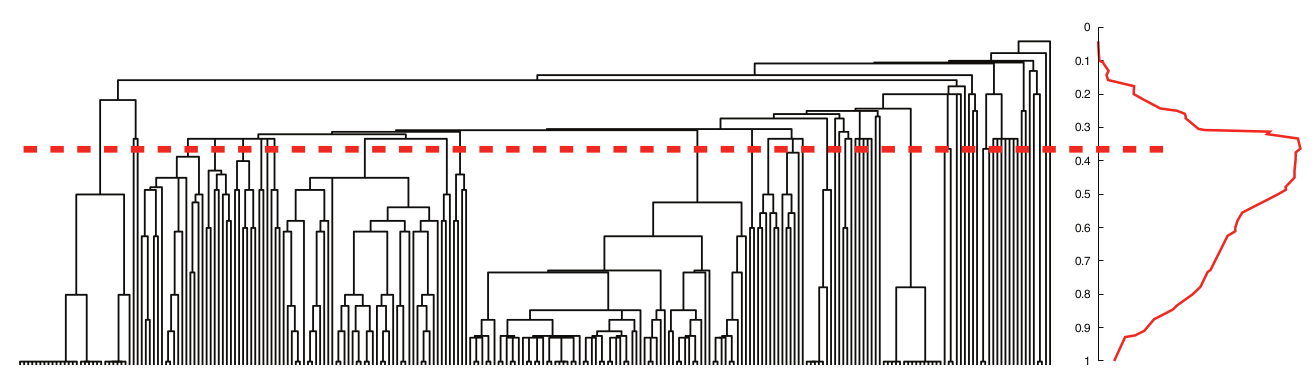
\includegraphics[clip,width=0.96\textwidth]{figures/figure0.png}
  \caption[Example of a full link dendrogram (left) and partition density (right)]%
  {Example of a full link dendrogram (left) and partition density (right), borrowed from~\cite{ahn2010link}.}
  \label{fig:hlc_density}
\end{figure}

The output of
cutting is a set of node clusters, where each node can participate in
multiple communities.

\subsection*{Least Absolute Shrinkage Selector Operator (LASSO)}

LASSO is a
regularized linear regression technique. By combining a regression
model with a procedure of contraction of some parameters towards $0$,
LASSO imposes a restriction (or a penalty) on
regression coefficients. In other words, LASSO solves the least
squares problem with restriction on the $ L_1$-norm of the coefficient
vector. In particular, the approach is especially useful in scenarios where the number
of variables $ c $ is much greater than the number of
samples $ m $ (i.e., $ c \gg m $).
\vspace{0.5cm}

Consider a dataset of $m$ samples, consisting each
of $c$ covariates and a single outcome. Let $y_i$ be the outcome and
$x_i := (x_{i1},...,x_{ic})$ be the covariate vector for the $i$-th
sample. The objective of LASSO is to solve
%
\begin{equation}
\min \left\lbrace\sum_{i=1}^{m}{\left( y_i-\sum_{j=1}^c{\beta_j
    x_{ij}}\right)^2} \right\rbrace \quad , \quad \textrm{subject to}
\quad \sum_{j=1}^c\abs{\beta_j}\leq s.
\end{equation}

where $s$ is the regularization penalty. 
Equivalently, in the Lagrangian form, LASSO minimizes

\begin{equation}
  \sum_{i=1}^{p}{\left( y_i-\sum_{j=1}^c{\beta_j x_{ij}}\right)^2} +
  \lambda \sum_{j=1}^c\abs{\beta_j}
\end{equation}
%
where $\lambda \geq 0$ is the
corresponding Lagrange multiplier. Since the value of the regularization
parameter $\lambda$
determines the degree of penalty and the accuracy of the model,
cross-validation is used to select the
regularization parameter that minimizes the
mean-squared error.


% Model framework - similar to materials and methods, but with more paragraph
% continuity

\subsection*{Framework Conception and Configuration}

As mentioned before, the functionality of a protein strongly depends on its 3D structure, 
so that changes in its conformation (mutations) can affect how a protein interacts with its 
surroundings \cite{Sikosek2014Prot}. In this aspect, $A_G$ gives intrinsic information 
about complementarity between pairs of proteins and hence paths on the protein network are 
relevant for the prediction task. 

The proposed framework for prediction of protein-protein interactions consists of the
combination of the path counting metrics along with the vector representations of the
edges of the network (node2vec embeddings). Namely, the path counting metrics are either 
the counting of paths of length 2 (matrix $A_G^2$), the counting of paths of length 3 
(matrix $A_G^3$) or the degree-normalized counting of paths of length 3 (matrix $L_3$). 
The information retrieved from these matrices will be addressed from now on as A2, A3 
and L3, respectively.

Figure \ref{fig:framework} shows the proposed framework for predicting protein-protein interactions. As the 
framework combines two sources of information, it consists of three processes: (a) Metrics 
calculation and initial predictions, (b) Node and edge embeddings and (c) Machine Learning 
prediction.

\begin{figure}[h]
\caption{\label{fig:framework}Framework scheme}
	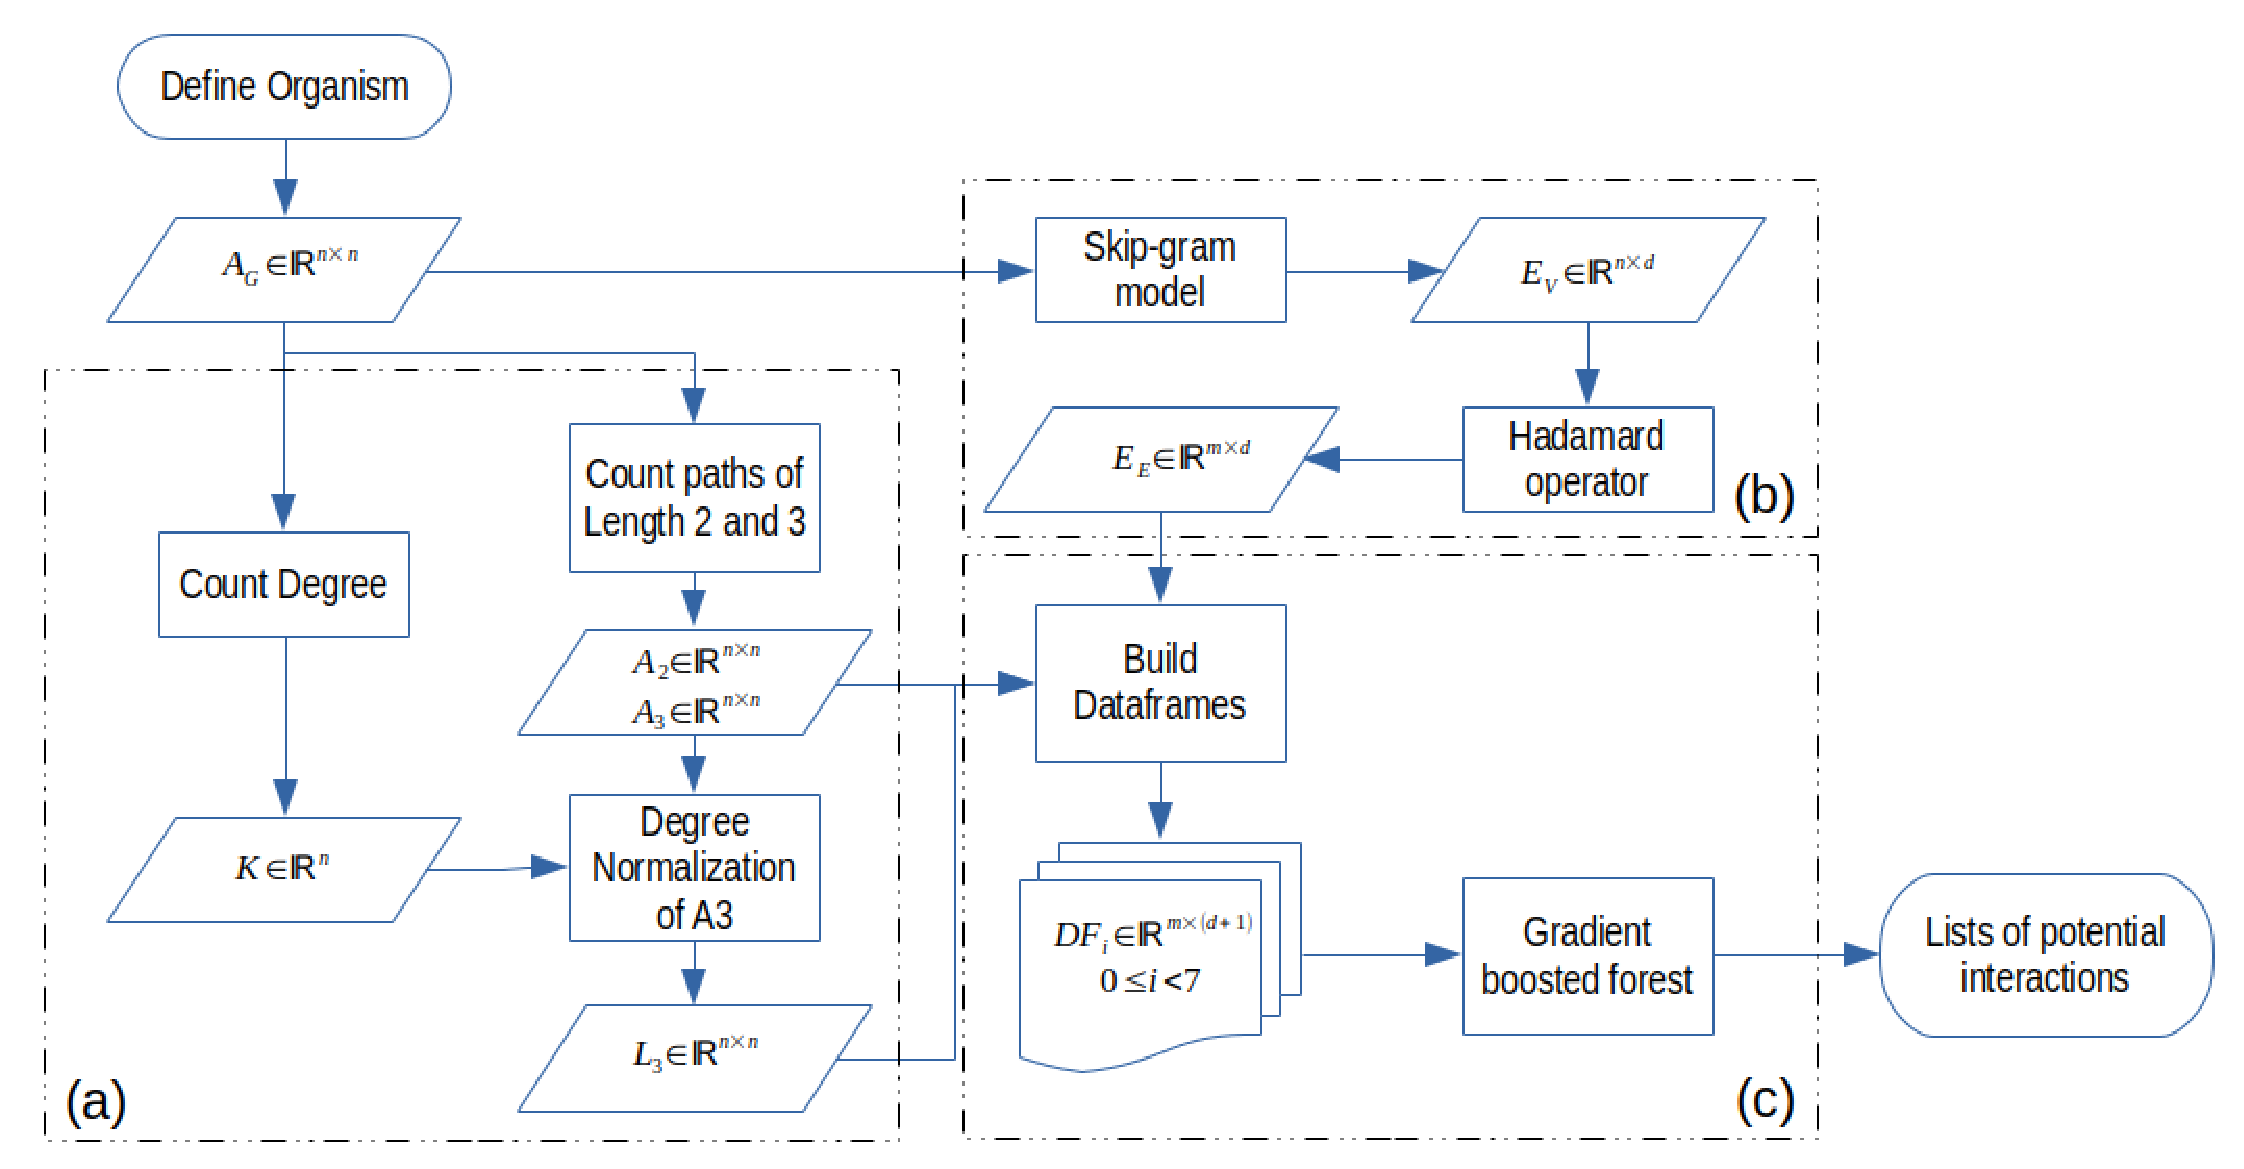
\includegraphics[width=\textwidth ]{figures/framework.eps}
\end{figure}

The input for the workflow consists of a representation of the connectivity of the network.
Online databases of protein-protein interactions usually report this information as an 
adjacency list with some additional attributes about the quality of this interaction. Namely, 
this data is represented as a list of pairs of identifiers and zero or more attributes for 
each pair. The framework only needs to know whether an interaction exists and therefore this 
additional information needs to be discarded in advance. In order to calculate optimally the
subsequent metrics, the framework creates the adjacency matrix $A_G$ out of the given list. 
Note that as no attributes from nodes or edges are added, the framework predicts based only 
on the intrinsic properties of the network related to connectivity. 

\subsubsection*{A. Metrics Calculation}
The goal of this stage is to build matrices $A2$, $A3$ and $L3$ which quantify, 
the number of paths of length 2, of length 3 and the degree-normalized count of 
paths of length 3, respectively. For this purpose, two calculations are done: 
counting the degree of each node ($k_i \in \mathbb{Z}$) and raising $A_G$ to the 
second to obtain $A2$. Finally, $A3$ and $L3$  are calculated simultaneously. 
Entries $L3_{i,j}$ of $L3$ can be calculated as 

\begin{equation}
  L3_{i,j}=\sum_{p,q\in V}\frac{{A_G}_{i,p}\cdot {A_G}_{p,q}\cdot {A_G}_{q,j}}{\sqrt{k_{p}\cdot k_{q}}}
\end{equation}

\subsubsection*{B. node2vec Embeddings}
The purpose of this step is to retrieve a vector representation of the network 
structure and thus be able to feed the Machine Learning model and improve its 
predictions. This is done using a state-of-the-art algorithm called node2vec, 
which is based on the word2vec technique to learn learn word associations from
a corpus of text. Instead of sentences, node2vec uses 
random walks from each node in order to construct a skip-gram model and a neural 
network to learn features (embeddings) from the nodes\cite{Grover_2016}. These 
features consist of a $d$-dimensional vector representation of each node.
Since the framework aims to predict edges, these node embeddings are used as 
input for the Hadamard operator to calculate edge embeddings. Namely, the edge 
embedding of edge $c_i,j$ is calculated as the element-wise product of each 
component of the node embeddings for nodes $i$ and $j$. $d$ is chosen as 16.

\subsubsection*{C. Machine Learning Prediction}
Finally, this stage aims at gathering information from the previous steps to 
enrich the prediction of a Machine Learning (ML) model and improve its results. 

The selected implementation for this prediction problem is XGBoost, which 
uses gradient boosted decision trees to learn whether an interaction is feasible. 
The first step in this process is to combine the two sources of information into 
Dataframes for each of the metrics: for each edge, the information from one of the 
metrics (A2, A3 or L3) is appended to the vector representation of $d$ dimensions 
from node2vec, resulting in 3 different tables. Dataframes including only one 
source of information (each metric or node2vec data) are also generated and 
fed to XGBoost for comparison.

For each metric, the initial prediction in step A is used to train the supervised 
ML model 


\subsection*{Framework Evaluation on the Human Interactome}

As the first step in the evaluation of A2, A3 and L3 metrics to assess link
prediction, the full calculation and ranking of all predictions was
carried out. The results for the analyzed human interactomes (\emph{HI-II-14}
and \emph{HI-TESTED}) is shown in Figure \ref{fig:HI1}, in which
the x axis represents a rank position $k$ and the y axis displays
the precision for the top $k$ predictions of each method, when assuming
interactome \emph{HI-III} as the validation set. 
	
\begin{figure}[h]
\caption{\label{fig:HI1}Methods Comparison for \emph{HI-II-14} and \emph{HI-TESTED}}
	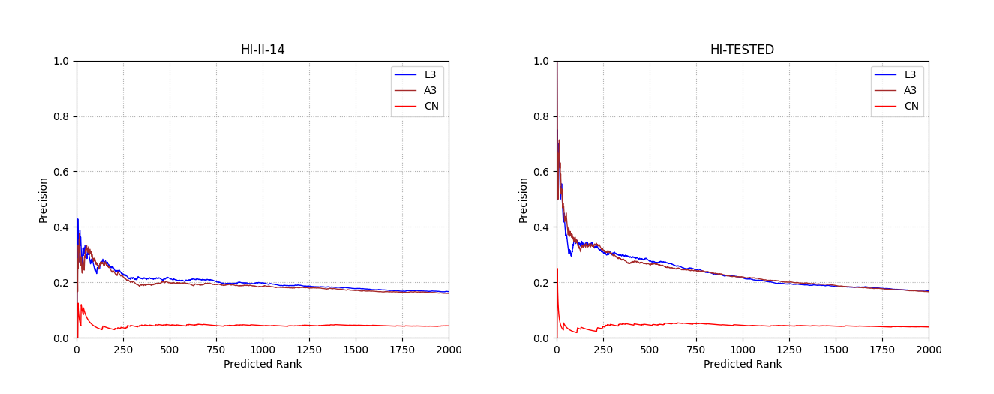
\includegraphics[width=\textwidth ]{figures/figure2.eps}
	%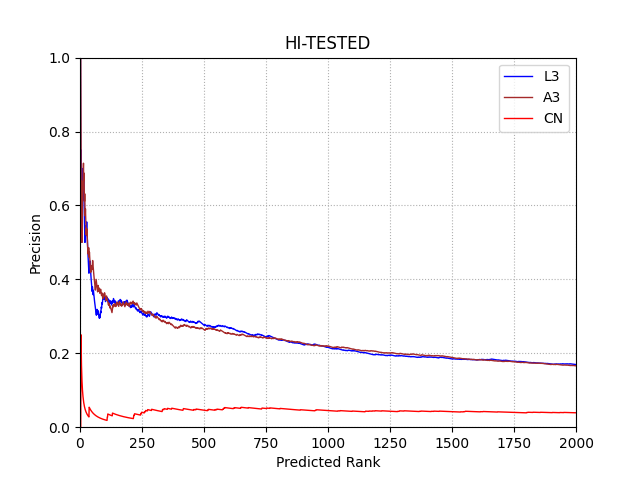
\includegraphics[width=0.7\textwidth ]{../hi-tested.txt.}
\end{figure}

As it can be inferred from the plots, L3-based predictions outperform
their $A{{}^2}$ counterparts. Results also show that L3-score and
$A^{3}$predictions follow a very similar trend.

However, the interest of this study is to assess if Machine Learning can boost
the overall performance on the prediction, so the proposed procedure
is adapted to the human interactome data: Instead of having to remove
a fraction of edges from the network in order to predict and validate,
the prediction network and the validation networks are given beforehand.
The rest of the procedure is carried out as mentioned above.
Table \ref{T1} presents the results for the combinations of Node2Vec
with each feature.

\begin{table}
\caption{\label{T1}Summary statistics for human interactomes}
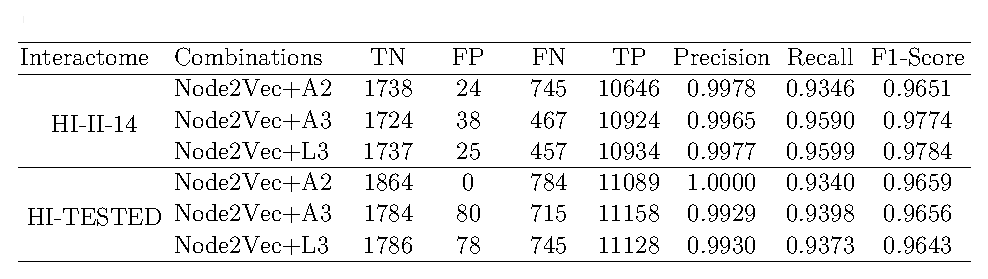
\includegraphics[width=1\columnwidth]{figures/T1}
\end{table}

In general, performance of all models is above 0.96 in terms of F1-Score.
Although marginally, the A2 feature-enriched model for HI-TESTED performs
better than their counterparts based on paths of length 3. The opposite
is also true for HI-II-14: models enriched with L3 and A3 features
perform better than their A2 counterpart. Results for the Interactome
\emph{HI-II-14} with Node2Vec and each metric are presented in Figures
S\ref{HI1}, S\ref{HI2} and S\ref{HI3}. It can be seen that for
\emph{HI-II-14}, A2 performs marginally better than L3 when comparing
precision but worse in terms of recall, although all metrics have
AUC values of 0.99.

On the other hand, the interactome \emph{HI-TESTED} was assessed with
the same methodology as \emph{HI-II-14} and results are shown in Figures
S\ref{HI1-1}, S\ref{HI2-1} and S\ref{HI3-1}. For this interactome,
A2 performs better in terms of false positives than A3 and L3, but
in terms of false negatives, A3 actually performs better that A2 and
L3. In terms of AUC, metrics results are indistinguishable. 

An interesting assessment from this human datasets can be observed
when looking at the importance plots, which show a very biased influence
of the handcrafted features. Figure \ref{F8-importance-H1} shows
this behavior for the \emph{HI-II-14} dataset, which is very similar
to \emph{HI-TESTED} (Figure S\ref{F8-importance-H2}).

\begin{figure}[h]
\noindent \begin{centering}
\caption{\label{F8-importance-H1}Importance gain plots for \emph{HI-II-14}}
\par\end{centering}
\begin{centering}
\includegraphics[width=0.48\columnwidth]{figures/Human/Imp\lyxdot A2\lyxdot 1\lyxdot eps}\includegraphics[width=0.48\columnwidth]{figures/Human/Imp\lyxdot A3\lyxdot 1\lyxdot eps}
\par\end{centering}
\centering{}\includegraphics[width=0.48\columnwidth]{figures/Human/Imp\lyxdot L3\lyxdot 1}
\end{figure}

%\section*{Results}
\section*{Identifying Potential Saline Stress Responsive Genes in Rice}
\label{sec.case}

This section presents a case study, applying the approach introduced in 
\hyperref[sec.framework]{the Workflow} section, to identify genes in
\textit{Oryza sativa} that respond to saline stress.
\vspace{0.5cm}

The RNA-seq data are available from the
GEO database \cite{clough2016gene} (accession
number GSE98455). It corresponds to $n_0=57\,845$ gene
expression profiles of shoot tissues measured for control and
salt conditions in $m=92$ accessions of the Rice Diversity Panel 1~\cite{eizenga2014registration},
with $r=2$ biological replicates. A total of $p=3 $ phenotypic traits
are used: shoot $K$ content, root biomass, and shoot biomass. These
traits were measured for the same $92$ genotypes, under control and
treatment conditions, and can be found in the supplementary
information for~\cite{campbell2017allelic}.

\subsection*{A. Data Pre-processing}

DESeq2 normalization is applied to the raw data and the biological
replicates are averaged. Genes exhibiting low variance are
identified as those with ratio of upper quantile to lower quantile
smaller than $1.5$ and are removed from the normalized data. Genes
with low expression, corresponding to those having more than $80\%$
samples with values smaller than $10$, are also removed. After this
filtering process a total of $n_1 = 9\,414$ genes are kept for further analysis.
\vspace{0.5cm}

From the Log Fold Change matrix $L_0$, genes whose difference between
upper quantile and lower quantile is greater than $0.25$ are
removed. Therefore, the resulting matrix $L_1$ contains the log ratios
of $n_2 = 8\,928$ genes. The logarithmic ratios of the phenotypic data,
for the $92$ accessions and the $3$ traits, are also computed.

\subsection*{B. Construction of the Co-expression Network}

The Log Fold Change matrix $L_1$ is used to compute the corresponding
similarity matrix.  For this network, it is observed that $\beta=3$ is
the smallest integer such that the $R^2 \geq 0.8
$. Figure~\ref{fig:beta} depicts the degree distribution of the
similarity matrix (left) and the degree distribution of the adjacency
matrix (right), which is the degree distribution of a scale-free
network with $R^2 = 0.8$ with $\beta = 3$.
\vspace{0.5cm}

%figure 2
\begin{figure}[htbp]
  \centering
    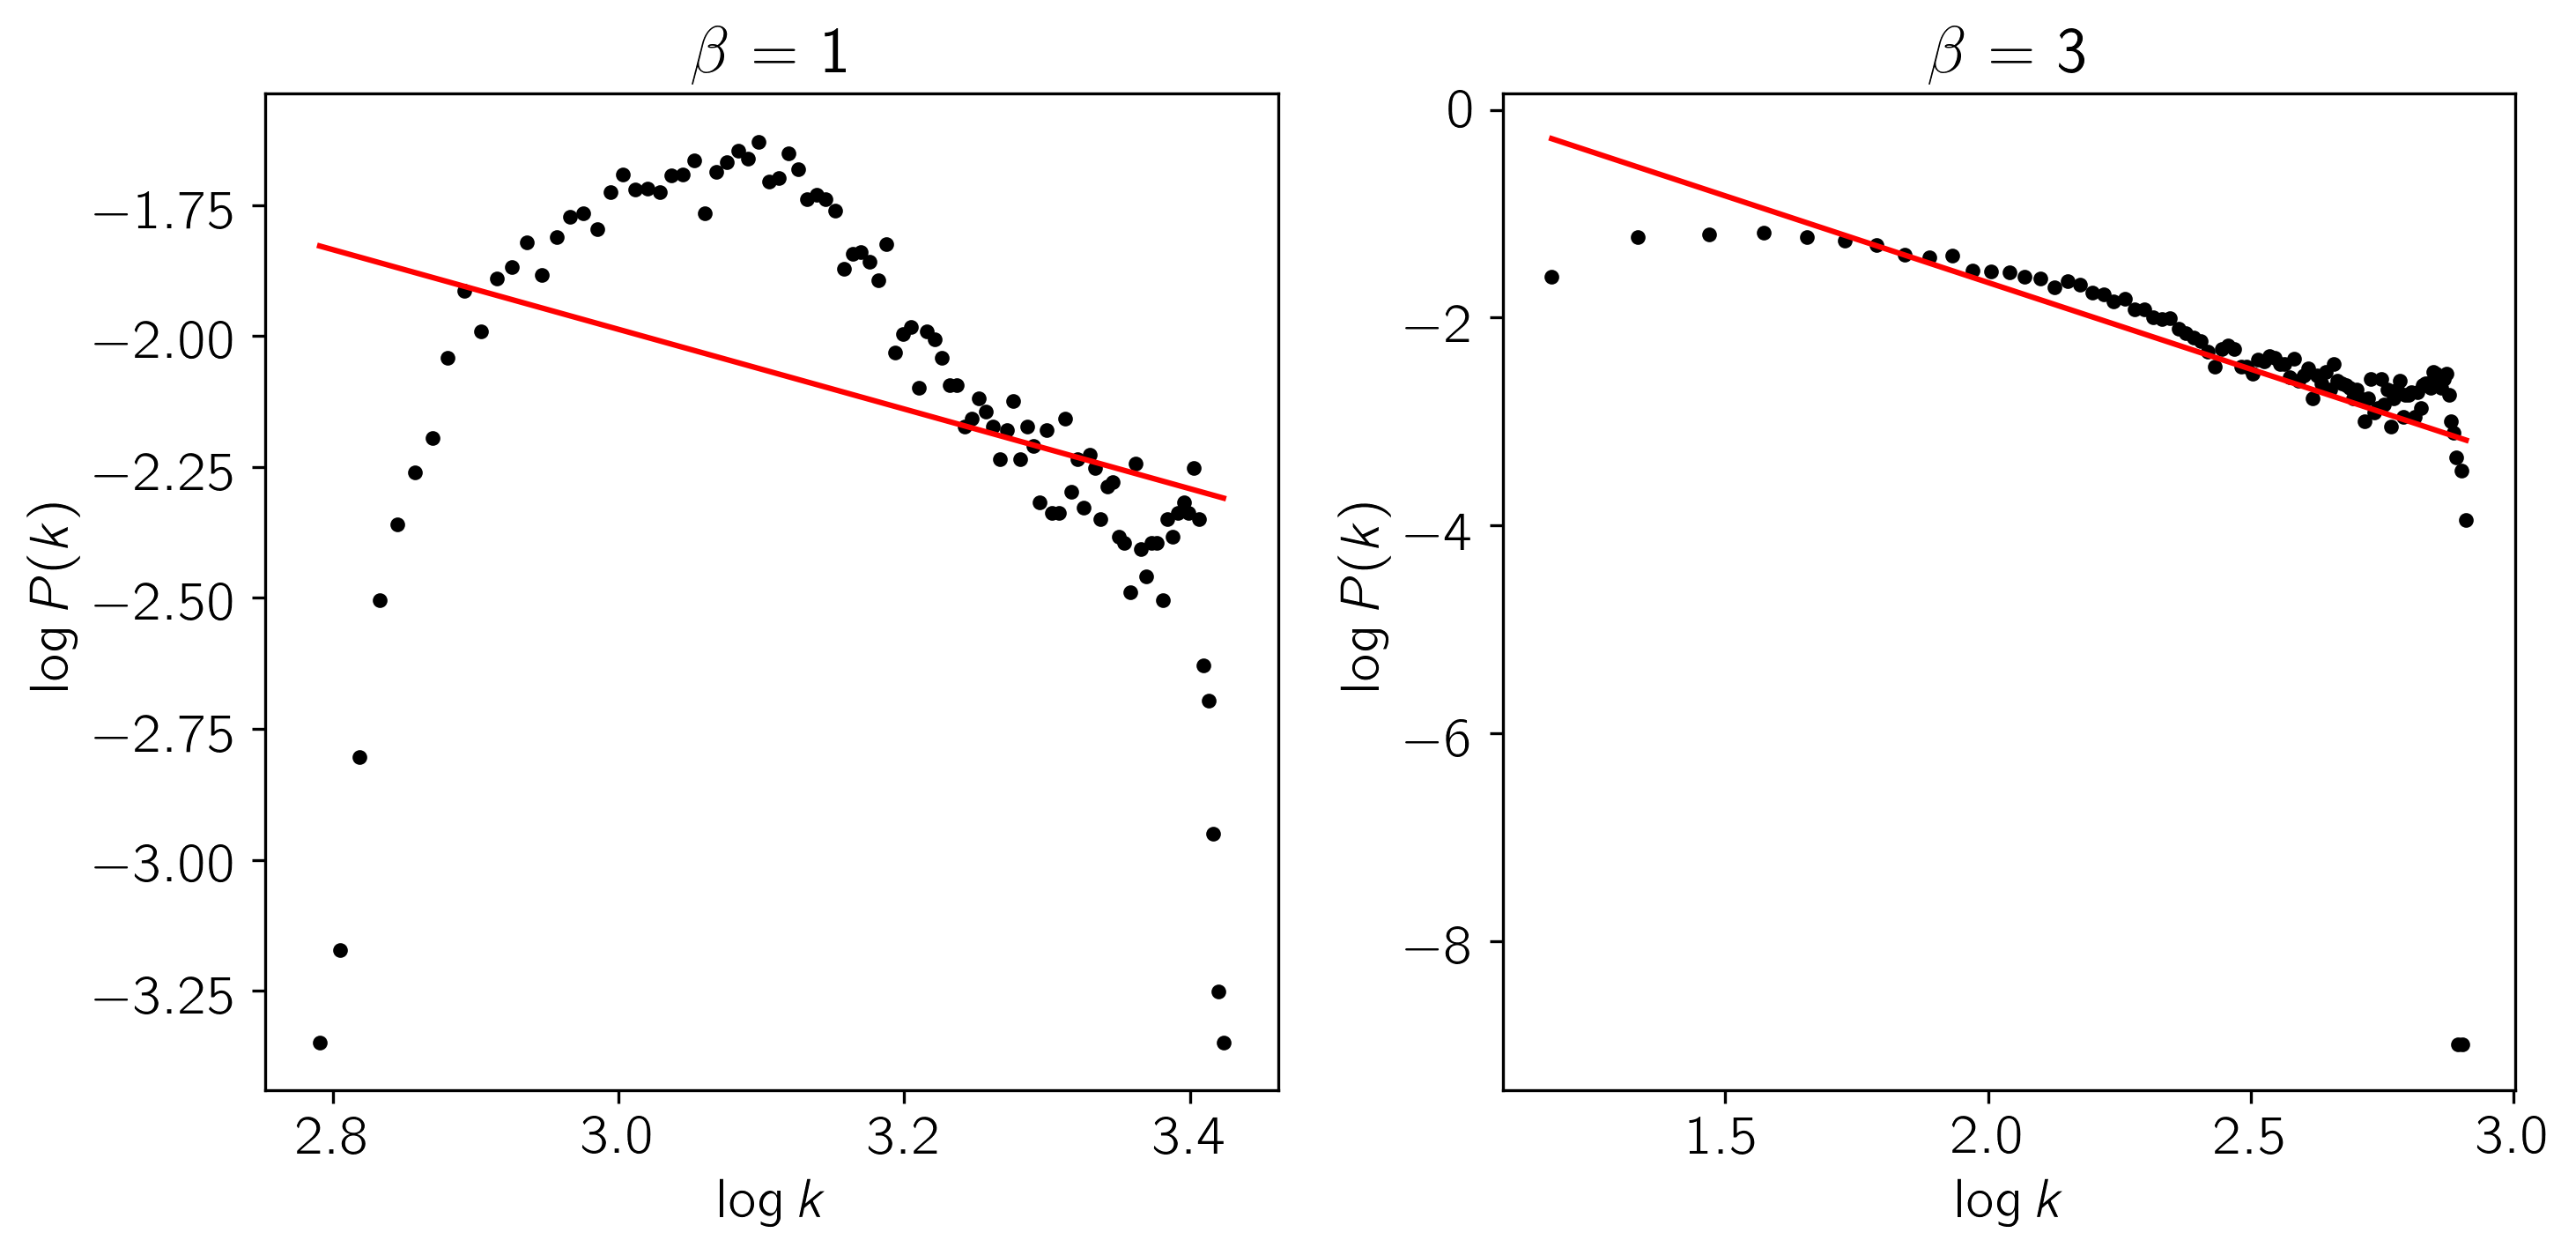
\includegraphics[clip,width=0.8\textwidth]{figures/figure2.png}
  \caption{Degree distribution of the network represented by $S$ (left) and $A$ (right).}
  \label{fig:beta}
\end{figure}

The resulting adjacency matrix $A$ represents a complete graph
$G=(V,E)$, with $|V| = 8\,928$ genes ($|E| = 39\,850\,128$ edges).

\subsection*{C. Identification of Co-expression Modules}

The adjacency matrix $A$ is transformed into an unweighted network
$\hat{A}$ applying the approach described
in~\cite{aoki2007approaches}. The cutoff value is set to $0.2$, 
based on the density of the network
combined with the decreasing number of nodes and edges with higher PCC
values. Thus keeping only the
connections above this threshold and removing any isolated nodes. The
resulting adjacency matrix $\hat{A}$ has $5\,810$ connected genes and
accounts for $614\,501$ edges.
\vspace{0.5cm}

After applying the HLC algorithm, a total of $4\,131$ genes are
distributed in $c = 5\,143$ overlapping modules of at least $3$
genes. Figure~\ref{fig:overlap} presents a histogram of the
overlapping percentage of these genes, measured as the proportion of
modules to which each gene belongs. The first bar of the histogram
represents the genes with zero overlap, corresponding to $28\%$ of the
total genes; the remaining $72\%$ represents the genes belonging to
more than one module.

%figure 3
\begin{figure}[htbp]
  \centering
    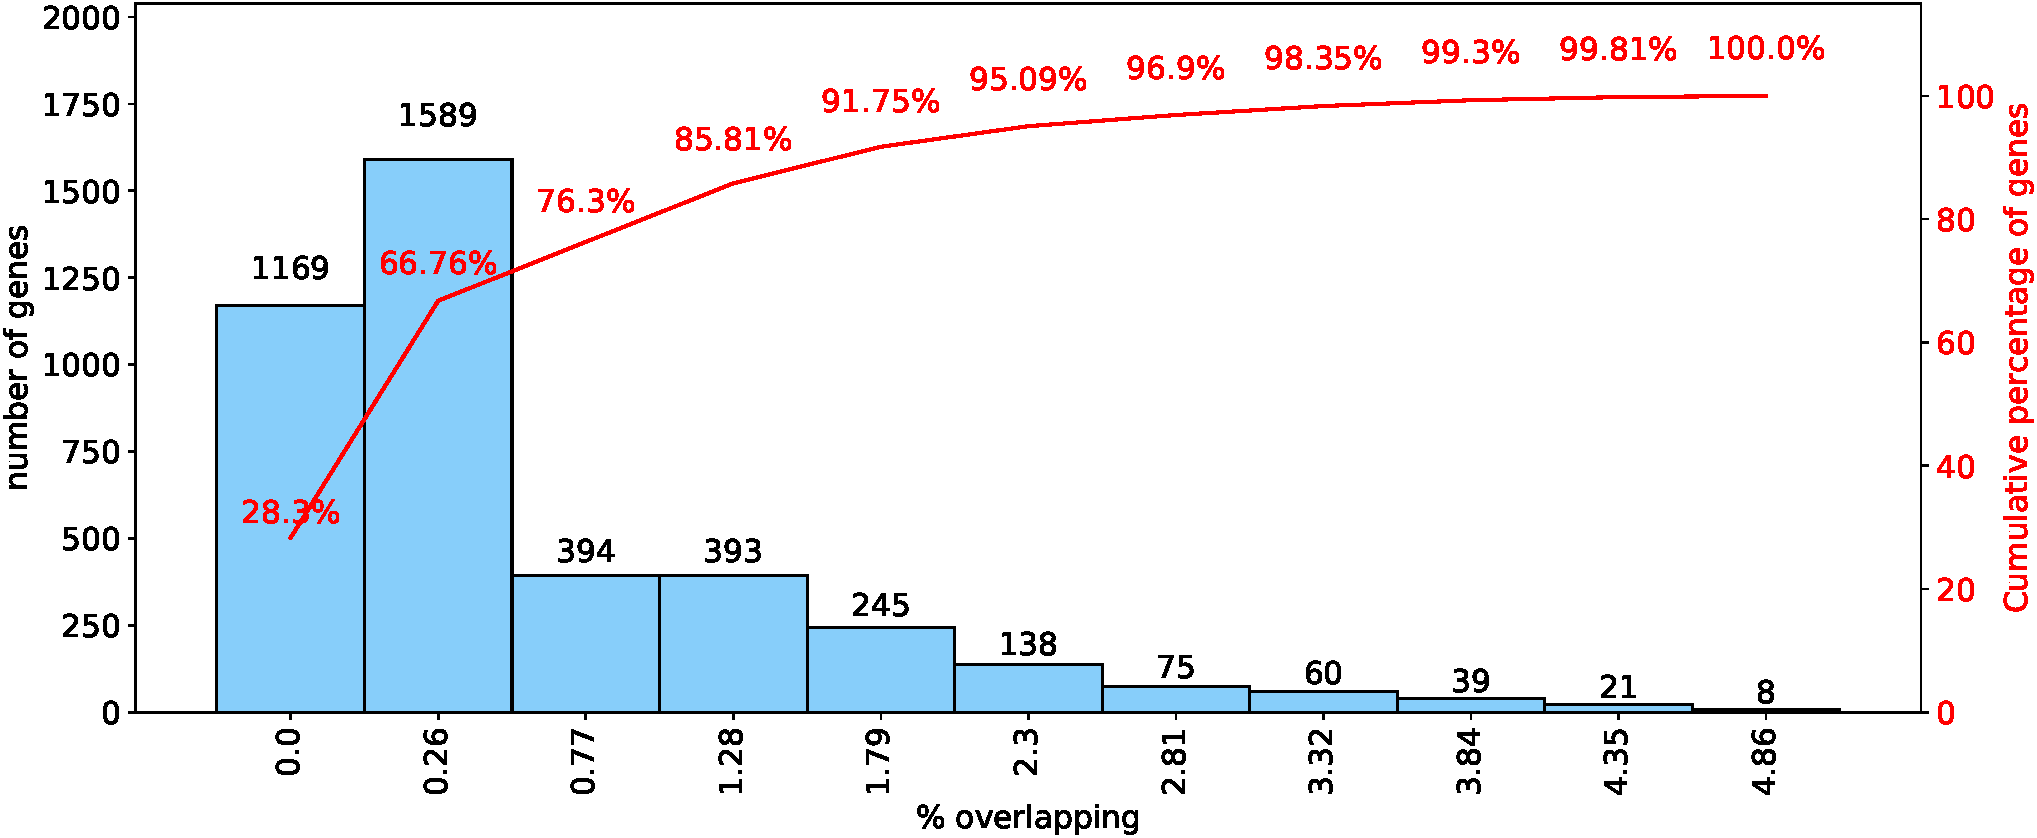
\includegraphics[clip,width=0.95\textwidth]{figures/figure3.pdf}
  \caption{Overlapping percentage of genes after applying HLC.}
  \label{fig:overlap}
\end{figure}

\subsection*{D. Detection of Modules Association to Phenotypic Traits}

The phenotypic traits under study are shoot $K$ content, root
biomass, and shoot biomass. Figure~\ref{fig:pdata} suggests that there
are significant differences in the values of these phenotypic traits
between stress and control conditions. This supports the working
hypothesis that these three variables represent tolerance-associated
traits in rice under salt stress.
\vspace{0.5cm}

%figure 4
\begin{figure}[htbp]
  \centering
    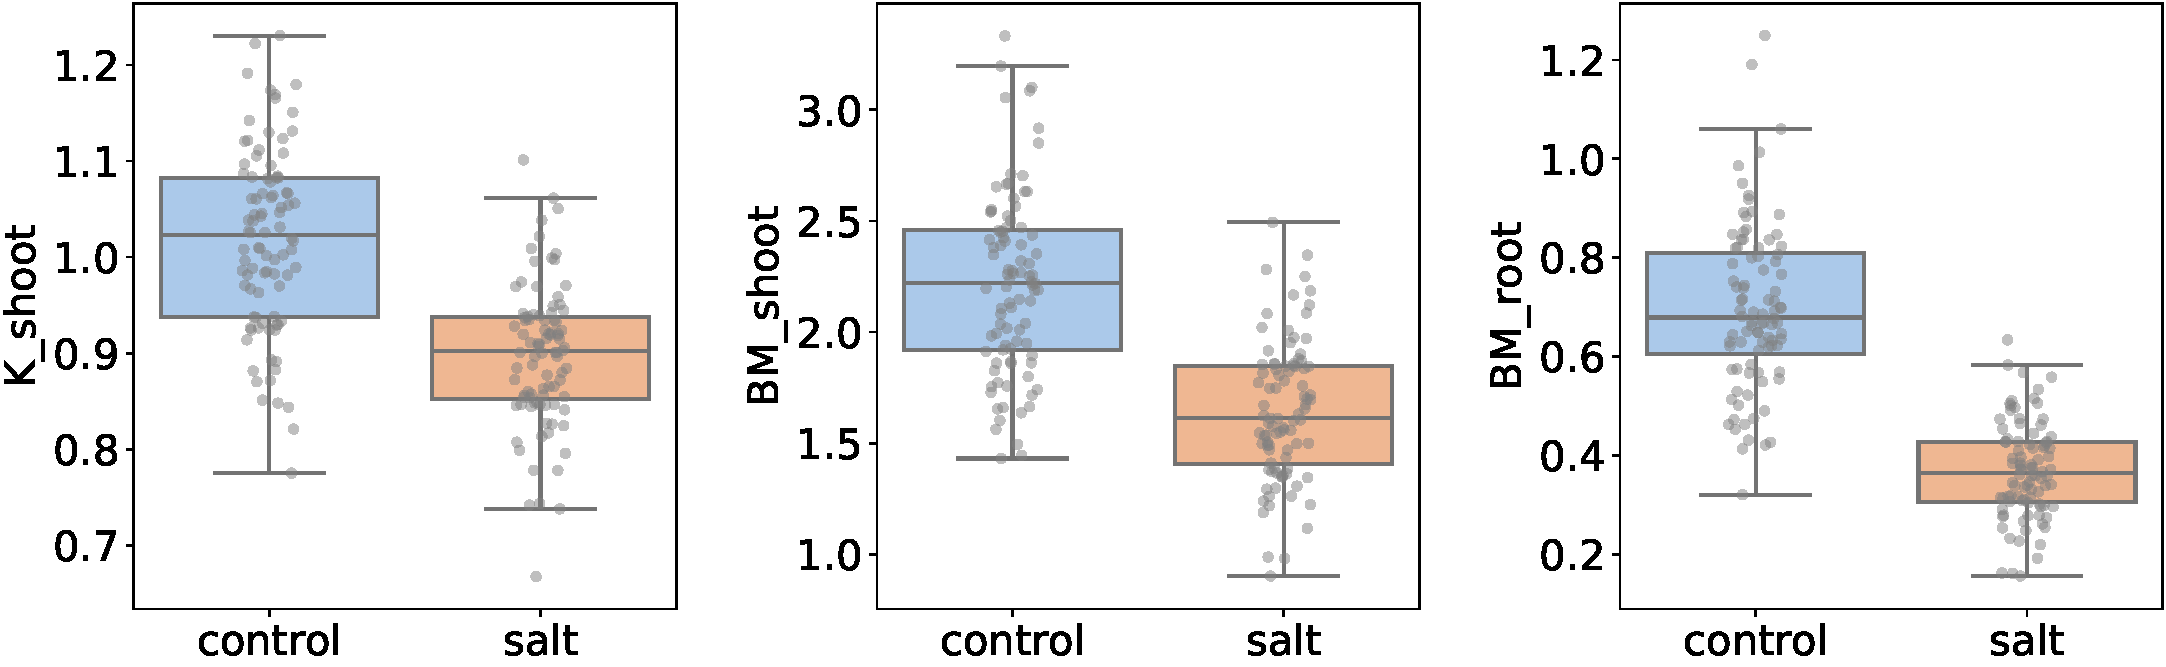
\includegraphics[clip,width=0.9\textwidth]{figures/figure4.pdf}
  \caption{Phenotipic traits distribution under control and salt stress.}
  \label{fig:pdata}
\end{figure}

Using the affiliation matrix $F$ derived from the HLC output and the
Log Fold Change matrix $L_1$, a matrix $M$ is built by computing the
eigengene for each of the $c = 5\,143$ modules. The LASSO technique is
applied by using each of the phenotypic traits as the outcome
variable, one at a time. As shown in Figure~\ref{fig:cross-val},
cross-validation is performed for each phenotypical trait in order to
select the corresponding regularization parameter $\lambda$ that
minimizes the mean-squared error.
\vspace{0.5cm}

%figure 5
\begin{figure}[htbp]
  \centering
    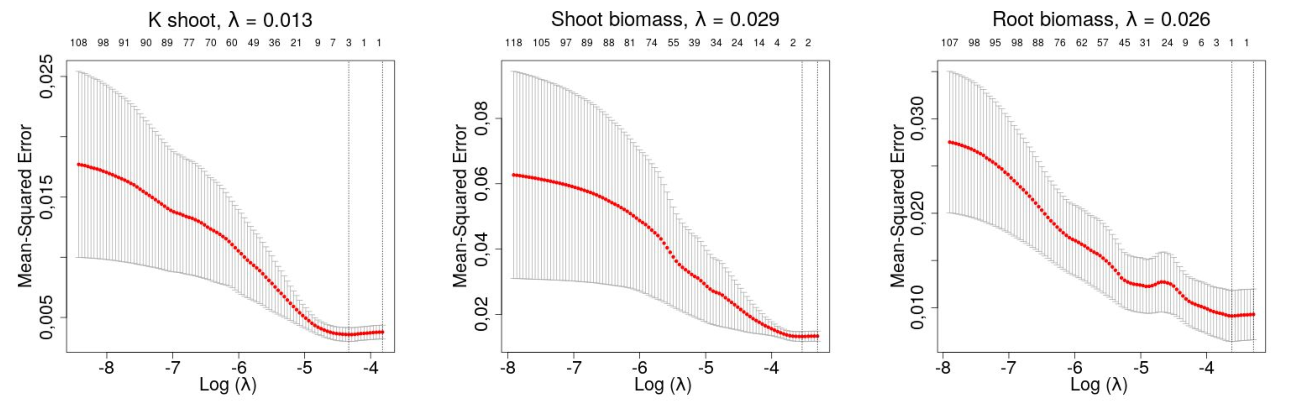
\includegraphics[clip,width=0.96\textwidth]{figures/figure5.pdf}
  \caption{Cross-validation of the LASSO regularization parameter
    $\lambda$, for each phenotypic trait.}
  \label{fig:cross-val}
\end{figure}

Finally, three LASSO models are adjusted by using the corresponding
$\lambda$ and phenotypical data with the eigengenes of matrix $M$. As
result, 6 modules are detected as relevant in the response to salt
stress in rice: 3 modules of 3 genes, each associated with shoot $K$
content; 2 modules of 3 genes associated with shoot biomass; and 1
module of 4 genes associated with root biomass (see
Figure~\ref{fig:final_genes}).

\subsection*{E. Gene Enrichment}

From the $19$ genes selected by LASSO, all but $3$ genes (the ones
associated to $K$ content), are also identified as deferentially
expressed ($|\ell_{ij}| \geq 2$) for at least one of the $92$
accessions. These genes are strong 
candidates target genes in rice.
%candidates as stress responsive genes to salt conditions in rice.
\vspace{0.5cm}

Figure~\ref{fig:final_genes} summarizes how from the initial
$n_0=57\,845$ genes, the proposed workflow identifies a reduced set of
$19$ genes. First, $48\,431$ genes are discarded after filtering the
normalized expression data $D_2$ and then $486$ additional genes are
discarded when filtering the Log Fold Change matrix $L_0$, to finally
arrive at $19$ genes, of which $16$ are differentially expressed.
\vspace{0.5cm}

% figure 6
\begin{figure}[htbp]
  \centering
    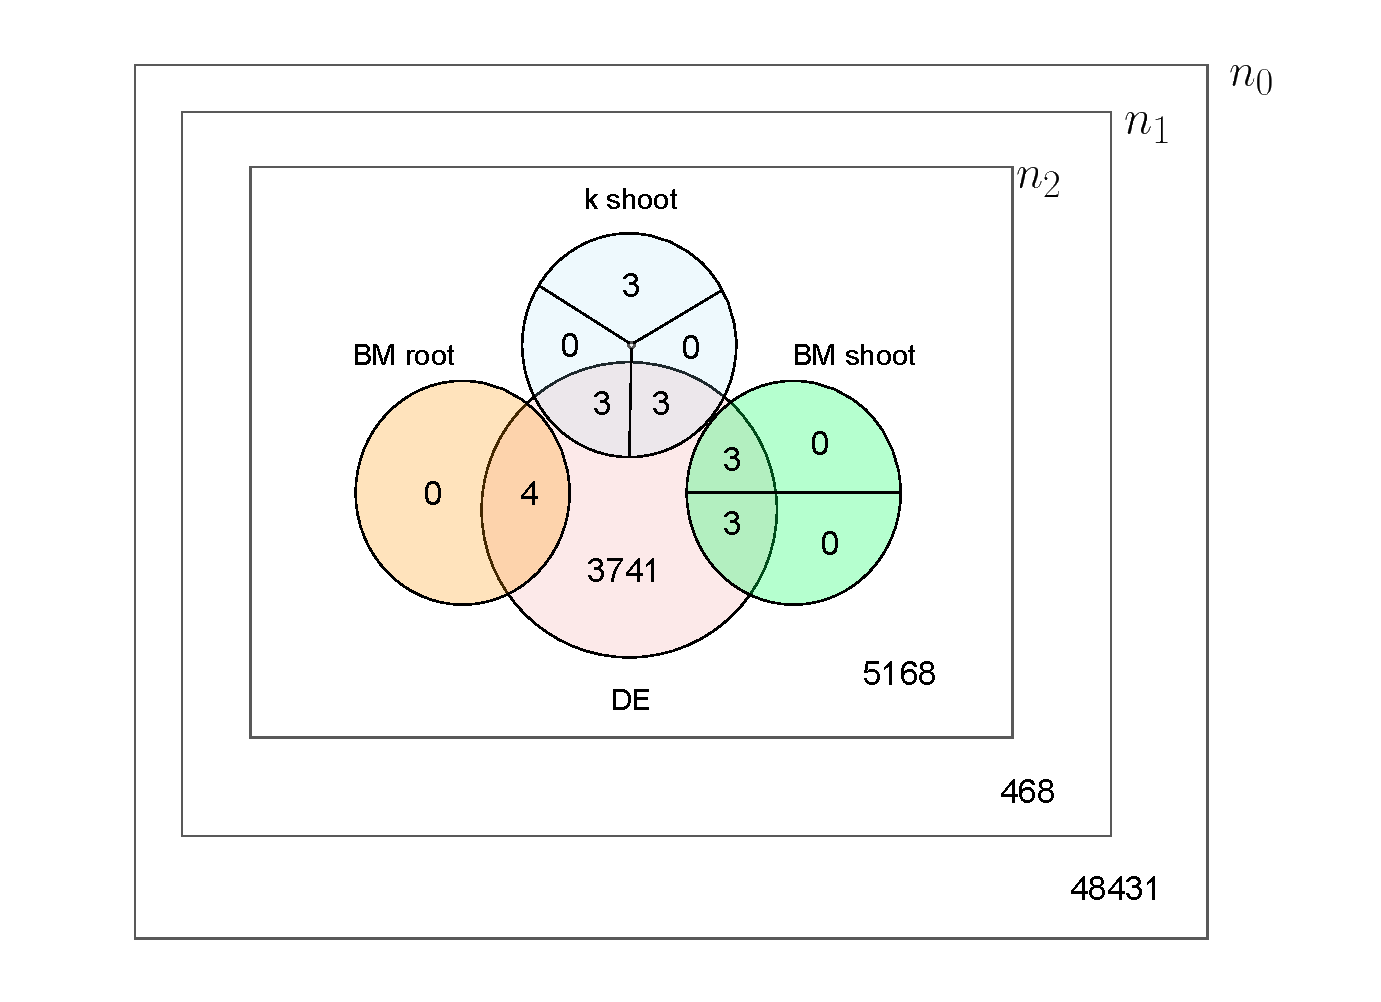
\includegraphics[clip,width=0.8\textwidth]{figures/figure6.pdf}
   \caption[Venn diagram for the case study in rice]%
   {Venn diagram representing the number of genes selected at
    different stages of the proposed workflow for the case study in
    rice.}
  \label{fig:final_genes}
\end{figure}

According to the Quickgo database, only $2$ of the $16$ differentially
expressed genes (both from the module related to shoot biomass) are
named and have an associated protein product: spermidine
hydroxycinnamoyltransferase 2 (SHT2) and lipoxygenase.
Figure~\ref{fig:3d} shows their corresponding 3D protein structures.
\vspace{0.5cm}

%figure 7
\begin{figure}[htbp]
  \centering
    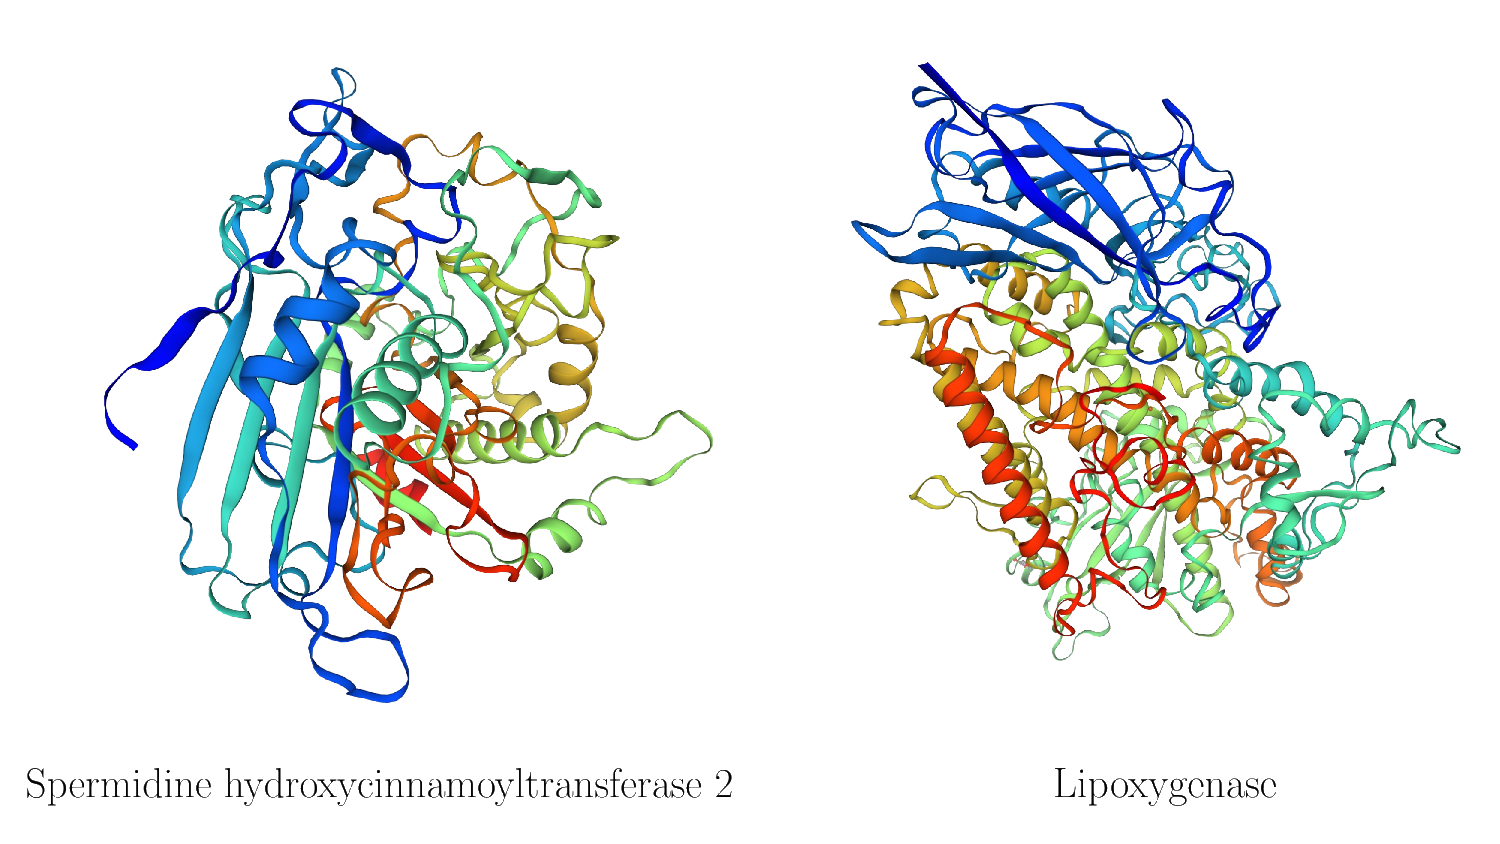
\includegraphics[clip,width=0.8\textwidth]{figures/figure7.pdf}
  \caption{3D protein structure of named genes selected by LASSO, borrowed from~\cite{szklarczyk2016string}.}
  \label{fig:3d}
\end{figure}

The Uniprot database~\cite{uniprot2018uniprot} reports, on the one
hand, that SHT2 contributes to the natural variation of
spermidine-based phenolamides in rice cultivars. On the other hand, it
is reported in~\cite{uniprot2018uniprot} that plant lipoxygenase may
be involved in a number of diverse aspects of plant physiology
including growth and development, pest resistance, and senescence or
responses to wounding. This protein is involved in the pathway
oxylipin biosynthesis, which is part of Lipid metabolism. Additionally,
previous studies
%
in~\cite{gupta2013plant,hou2015persimmon,mittova2002salt,peng2019novel,roychoudhury2011amelioration}
%
provide evidence of biological implications of sperimidine and
lipoxygenase in tolerance to salt stress in other plants or even in
rice cultivars.

As a conclusion, the results presented in this section suggest that
further studies are needed to elucidate the detailed biological
function of the remaining 14 genes that have not been named so far in
the literature.  They may have the potential to intervene in stress
responsive mechanisms to salt conditions in rice.


\section*{Concluding Remarks}
\label{sec.concl}

This manuscript provides a detailed description of a network-based
analysis workflow for the discovery of key genes responding to a
specific treatment in an organism. It links transcriptomic with
phenotypic data and identifies overlapping gene modules.
\vspace{0.5cm}

The proposed approach is inspired by the workflow suggested in the
WGCNA~\cite{langfelder2008wgcna}. Its main steps are the preprocessing
of the gene expression data, the construction of a co-expression
network, the detection of modules within the network, the relation of
modules with external information (e.g., phenotypic data), and the
enrichment of the identified key genes with additional information.
Both approaches are structured in a modular way, which allows
modifying and exploring different techniques in each step of the
workflow.
\vspace{0.5cm}

The proposed workflow is designed to integrate expression data
measured under two different conditions (namely, control and
treatment), unlike the usually co-expression-based approaches which
work with both conditions independently or consider only a single
condition. For this purpose, an approach similar to that proposed
in~\cite{du2019network} is used, where the control and treatment data
are compiled in a single matrix using the Log Fold Change
measure. Thus, the input to construct the co-expression network is not
the expression data, but instead the changes in the expression levels
from one condition to the other, making room for capturing the signal
of changes caused by the treatment.
\vspace{0.5cm}

An important feature in the proposed workflow is the module
detection technique. The co-expression network is computed, as in
WGCNA, until a scale-free network is obtained. In the proposed
approach, this network is then used to apply the HLC algorithm, a
clustering technique capable of detecting overlapping
communities. Several approaches of module detection from gene
expression have been proposed and were evaluated
in~\cite{saelens2018comprehensive}. Most of them focus mainly on
disjoint (non-overlapping) communities; the techniques described
dealing with overlaps are not clustering, but bi-clustering and
decomposition methods. It is well known that communities in real
networks, including biological ones, are likely
overlap~\cite{palla2005uncovering}. Thus, the approach presented
in this work can be seen as a generalization of the previous
approaches, such as WGCNA, with the potential to deal with genes
associated to multiple biological processes.
\vspace{0.5cm}

The approach was applied in a case study with rice under salt
stress. The results show a group of 14 genes, of which only $2$ of
them have been previously related to saline stress response in other
studies. As future work, other overlapping module detection and
selection techniques should be used instead HLC and LASSO,
respectively. The combination of these techniques would allow finding
target genes for future biological studies that evaluate their
potential as genes that respond to salt stress in rice, and other
crops and stresses. In-vivo laboratory experimentation needs to be
conducted to validate the findings of this paper in relation to
salinity stress.
\vspace{0.5cm}

Finally, the workflow is presented as a protocol capable of
considerably reducing the number of genes detected as relevant in the
response to stress of choice. Other traditionally used methods for
this purpose tend to generate a large list of candidate genes, thus
limiting subsequent efforts in experimental validation. In this sense,
the proposed workflow can help in reducing such efforts in time and
money invested by researchers in the experimental validation of
stress-responsive genes.


\begin{backmatter}
\section*{Acknowledgements}%% if any
Not applicable

\section*{Funding}%% if any
This work was funded by the OMICAS program: Optimización Multiescala In-silico de
Cultivos Agrícolas Sostenibles (Infraestructura y Validación en Arroz y Caña de Azúcar),
anchored at the Pontificia Universidad Javeriana in Cali and funded within the Colombian
Scientific Ecosystem by The World Bank, the Colombian Ministry of Science, Technology and
Innovation, the Colombian Ministry of Education and the Colombian Ministry of Industry 
and Turism, and ICETEX, under GRANT ID: FP44842-217-2018.

\section*{Abbreviations}%% if any
\textbf{HLC:} Hierarchical Link Clustering\\
\textbf{LASSO:} Least Absolute Shrinkage Selector Operator\\
\textbf{PCC:} Pearson Correlation Coefficient\\
\textbf{RNA-seq:} RNA sequencing\\
\textbf{SHT2:} Spermidine hydroxycinnamoyltransferase 2\\
\textbf{WGCNA:} Weighted Gene Co-expression Network Analysis

\section*{Availability of data and materials}%% if any
The datasets analysed during the current study are publicy available. They can be found in the following locations:
\begin{itemize}
\item RNA-seq data of salt stress in rice is available on the GEO (GSE98455).
\item Phenotypic data of salt stress in rice is a subset of the supplementary file 1 included in ~\cite{campbell2017allelic}.
\end{itemize}

\section*{Ethics approval and consent to participate}%% if any
Not applicable

\section*{Competing interests}
The authors declare that they have no competing interests.

\section*{Consent for publication}%% if any
Not applicable

\section*{Authors' contributions}
J.F. and C.R. proposed the original idea. 
J.F. provide advice on algorithms concepts and implementation.
C.R. structured the methodology and performed the analysis. 
C.R., J.F., and H.C.R. wrote the manuscript.
All authors read and approved the final manuscript.

\end{backmatter}

%\bibliographystyle{splncs04}
\bibliographystyle{bmc-mathphys}
\bibliography{biblio}

\end{document}

